\chapter{The Ensemble Nature of the Schr\"{o}dinger Equation and its Wavefunction, and a New Universal Action Mechanics}\label{chap27}

%\Authorline{N.G.Deshpande// Professor of Physics, University of Oregon}

\begin{center}
\textbf{C. S. Unnikrishnan}\\
\textbf{\textit{Tata Institute of Fundamental Research, Homi Bhabha Road, Mumbai 400005}}
\end{center}

\begin{center}
(Date textdate)\\

\medskip

Abstract
\end{center}


All researchers of quantum mechanics assume that the Schr\"{o}dinger equation is the equation for
dynamics, akin to Newton's equation of motion or the Hamilton-Jacobi equation for the evolution
of action. The wavefunction $\psi(x)$ is assumed to be some way associated with a single particle,
or a single quantum history. Hence, Born's ad hoc interpretation is necessary to connect the psi-function to the statistical results of an ensemble of observations. Here I show that the Schr\"{o}dinger
equation is not the equation for dynamics, but it is in fact the equation for the evolution of
the ensemble probability density $\rho(x)$, written in terms of the single valued square root $\chi(x)$
of the probability density, \textit{with the constraint that $\rho(x)$ is that of a dynamical system}. It then
follows that the Born's rule is an exact relation $\chi \chi^{\ast} \equiv \rho$, by definition. This implies that a
matter-wave is absent in quantum mechanics; $\psi(x)$ is not the matter-wave. Neither is it the
representative of a single quantum history. The psi-function is an ensemble averaged quantity.
The true dynamical equation is a modified Hamilton's equation for the action-wave $\zeta(S)$. This
completes the Hamiltonian dynamics to a universal dynamics, with the encompassing uncertainty
relation $\Delta S \geq \hbar$. These findings define the kernel of quantum dynamics without any of the
foundational problems of interpretation or ontology, while retaining all the statistical results of
quantum mechanics.

\section{Introduction}

``\textbf{It will be impossible to answer any one question completely without at the
same time answering them all}", P. A. M. Dirac, Proc. Roy. Soc. Lond. A, Vol. 114,
243 (1927).

The Schr\"{o}dinger equation marked a decisive milestone of modern quantum mechanics
(QM), after two decades of isolated results of importance in atomic physics. The equation
was also considered as the completion of non-relativistic QM, apart from the addition of the
Born's rule. Its more detailed structure, compared to Heisenberg's earlier breakthrough of
finding the `rule of quantization', made it the basis of most discussions and the calculations
of the theory. Schr\"{o}dinger arrived at the first order equation for the time evolution of
`something like a wave' after many steps, spread over four papers in 1926, starting with a
second order wave equation that resembled conventional second order wave equations [1].
The differential equation was written for the time evolution of the ``wavefunction", which was
notionally related to, and inspired by, de Broglie's matter-wave. The Schr\"{o}dinger equation
is
\begin{equation*}
i \hbar \frac{\partial \psi (x)}{\partial t} = \hat{H} \psi (x) \tag{1}
\end{equation*}
where $\hat{H}$ is a differential operator corresponding to the Hamiltonian of the system. However,
as well known, the wavefunction or the `psi-function' $\psi (x)$ cannot be interpreted as a physical
entity is real space, though it is a function of the $3N$ coordinates of the $N$ particles in the
quantum system. It does not directly represent the material particle or a wave corresponding
to the particle, evolving in real space. Thus, the complex valued psi-function remains as
much of a mystery now as it was about a century ago. The only additional interpretational
insight was M. Born's proposal that the absolute square of the $\psi$-function, $\psi(x) \psi^{\ast}(x)$, is to
be equated to the probability density $\rho(x)$ for evaluating the statistical results of all possible
observations of the system.

Subsequent formal developments clarified the mathematical structure of QM and clearly
delineated how to use the theory for the precise calculations of ensemble averaged quantities
of interest. The generalization to the Pauli equation for the two-component `spinor' psi-
function and the further generalization to the relativistic case with the invention of the Dirac
equation completed the quantum theory of particles. The comparison with experimental
observations, and the excellent empirical agreement in every known case, suggest that the
present QM is the correct statistical description of physical effects in the microscopic atomic
world, to the tiniest scales.

I intend to take a close look at the Schr\"{o}dinger equation, to reveal its true structure
and meaning, including the real nature of the elusive `psi-function'. I will show that \textit{the
Schr\"{o}dinger equation is not the equation for dynamics}. Rather, it is the equation for the
time evolution of a probability density, written in terms of its single valued square root, with
the constraint that the probability density corresponds to the dynamics of an ensemble of
particles. In other words, the Schr\"{o}dinger equation is an ensemble equation, and not the
equation for the single particle or single quantum history. This drastically changes the basis
for the entire understanding of quantum mechanics, hitherto followed in all approaches
to the interpretation of the theory. Then the question arises immediately, what then is
the core equation of quantum dynamics?! The correct equation for dynamics is found by
modifying and completing Hamilton's equation for the evolution of the action S, to a new
equation for the true ``wavefunction of action" $\zeta(S)$, which describes the universal dynamics
of particles at all scales and all velocities \cite{chap27-key2}. The new dynamics reveals the reason for the
intrinsic uncertainty, with the new general relation $\Delta S \geq \hbar$. It is argued, from empirical
considerations, that there is no matter-wave, and that matter itself does not have any wave
property. The sole `wave' in quantum mechanics, and indeed in all mechanics, is the `action-
wave'. It is shown, with explicit demonstrations and calculations, that the new mechanics
solves the vexing problems of the collapse of the quantum state and quantum measurement,
as well as the alleged problem of nonlocality in multi-particle correlations. In addition, the
new mechanics is free of the divergence of zero-point energy in the vacuum wave modes.
With these clarifications and features, quantum mechanics seems completed, both in its
structure and in its physical interpretation, a century after its formulation. Now, we can
not only calculate with quantum mechanics, but also understand the dynamics consistently
and causally, without conceptual clashes or ambiguities.

\section{The Schr\"{o}dinger Equation}

Schr\"{o}dinger started his exploration of a wave equation, for the matter wave conjectured
by de Broglie, with the familiar differential equation for waves,
\begin{equation*}
\nabla^2 \psi (x,t) - \frac{\partial^2 \psi (x,t)}{u^2 \partial t^2} = 0 \tag{2}
\end{equation*}
where the velocity $u = E/ [2m(E - V )]^{1/2}$. With the time dependence of the $\psi$-function
that obeys the relation $E = h\nu$ limited to $\psi(t) \infty \exp \pm i2\pi \nu t$, one gets $\ddot{\psi} (t) = -4 \pi^2 E^2 \psi /h^2$.
The resulting equation with the Coulomb potential in the Hydrogen atom $V (r) = e^2 /r$,
\begin{equation*}
\nabla^2 \psi + \frac{8 \pi^2 m}{h^2} (E + e^2 / r) \psi = 0 \tag{3}
\end{equation*}
\textit{did provide the Bohr spectrum of Hydrogen atom} \cite{chap27-key1}. Since the interpretation of $\psi$ as the
matter wave of the single electron around the nucleus sort of fitted what the equation was
suggesting, the initial interpretation of the Schr\"{o}dinger equation as a wave equation repre-
senting dynamics, and its wavefunction as the matter wave in space, was widely influential.
This general identification of matter as a dual entity, \textit{as both a particle and a wave}, determined the rest of the history of the physical interpretation of QM. However, it may be noted that there was no compulsion from experiments to equate the particles with a wave,
both propagating in space; what was empirically required was the association of only the
dynamics (motion) of the particle, and the material particle itself, with an unobservable
wave-like entity, with the periodicity $\hbar$ in the action $S$.

What was Schr\"{o}dinger's route from the equation
\begin{equation*}
\nabla^2 \psi(x,t) + \frac{2m}{\hbar^2} (E-V) \psi = 0 \tag{4}
\end{equation*}
to the final Schr\"{o}dinger equation? Stated concisely, he eliminated the quantity $E$ in the
equation by writing the time derivative $\psi(t) = 2\pi i E \psi /h$. Then we get
\begin{equation*}
\nabla^2 \psi (x,t)  + \frac{2m}{\hbar^2} [-i \hbar \dot{\psi} (t)] - \frac{2m}{\hbar^2} V_{\psi} = 0 \tag{5}
\end{equation*}
which is the Schr\"{o}dinger equation
\begin{equation*}
i \hbar \frac{\partial \psi (x,t)}{\partial t} = - \frac{\hbar^2}{2m} \nabla^2 \psi (x,t) + V \psi  \tag{6}
\end{equation*}

Clearly, the logical path followed was not one that guaranteed, or even suggested, an
equation of dynamics. Note that there was no relation made between the combination
$(\nabla^2 + V )$ and an operator corresponding to the Hamiltonian of the system. The total energy
was in fact represented by the time derivative because that was obtained by replacing $E$
with $\dot{\psi}$, after assuming harmonic solutions. Also, one just assumed its general validity for
time-dependent potentials as well. Schr\"{o}dinger invoked `success' as the justification for the
procedure. However, the price paid for the success was that he had to hesitantly abandon
any acceptable physical interpretation of the psi-function and the wave equation. The first
order time derivative may remind us of the first order derivative in the celebrated Hamilton's
equation (called the Hamilton-Jacobi equation) of the action,
\begin{equation*}
\frac{\partial S (x,p,t)}{\partial t} = - H \tag{7}
\end{equation*}

But this is misleading, because there is no obvious relation between the function $\psi$ and the
action S. The reason I retraced Schr\"{o}dinger's path to the final equation was to remind
that there is no direct correspondence between the action $S(x, p, t)$ and the wavefunction
$\psi(x, t)$ in spite of the fact that Schr\"{o}dinger derived much of the motivation and guidance
from Hamilton's work while formulating a wave equation for quantum dynamics. However,
the superficial resemblance, especially the first order time derivative, has been serving as a
misdirecting factor.

During his struggle to find a physical interpretation, Schr\"{o}dinger realized that only the
product $\psi(x) \psi^{\ast}(x)$ had any clear physical meaning; he saw $e|\psi|^2$ as representing the effective
charge density of a `fuzzy' electron. Even that was beyond an interpretation consistent
with the conventional notion of localized matter. It was only after Born's interpretation of
$\psi(x)\psi^{\ast} (x)$ as a probability density, rather than a real density of any physical quantity in
space, that one could claim a satisfactory structure in the theory of QM. Then, one got the
option to keep the particle as `point' matter, and $|\psi|^2$ as referring to the (statistical) ensemble
of particles. However, it also marks a missed opportunity for a complete understanding of
the new mechanics. If $\psi(x) \psi^{\ast} (x)$ is indeed the probability density, an evolution equation
for $\psi(x)$ should most naturally be related to the time evolution of the probability density,
rather than to the dynamics of a particle! And it is known that the time evolution of the
probability density of a closed ensemble is given by a first order partial differential equation
in time, called the equation of continuity or conservation,
\begin{equation*}
\frac{\partial \rho (x,t)}{\partial t} = - \nabla \cdot (\rho \upsilon) \tag{8}
\end{equation*}

This equation does not appear to be related to either the Hamilton's equation or the
Schr\"{o}dinger equation, especially with its first order spatial derivative. However, there are
two ways in which the second spatial derivatives are implicit in the continuity equation. One
is because the dynamical velocity $\upsilon$ is related to the action $S$ in the Hamilton's equation
by the relation $p = m \upsilon =\nabla S$. Another is when the statistical ensemble has a diffusion-
like behaviour, in which case the probability current is proportional to the gradient of the
probability density, $\rho \upsilon = - D \nabla \rho$. Then
\begin{equation*}
\upsilon = - \frac{1}{\rho} D \nabla \rho  = - D \nabla (l n \rho) \tag{9}
\end{equation*}


Thus, the evolution equation for the probability density in the general case is
\begin{equation*}
\frac{\partial \rho (x,t)}{\partial t} = - \nabla \cdot (\rho \upsilon) = - \nabla \cdot \left(\frac{\rho \nabla S}{m} - D \nabla \rho \right) = - \frac{\rho}{m} \nabla^2 S - \frac{1}{m} \nabla \rho \cdot \nabla S + D \nabla^2 \rho \tag{10} 
\end{equation*}

This has second spatial derivatives on the right. But it is not an equation for dynamics. It
is explicitly an equation for the statistical ensemble and the quantity $\rho (x, t)$ characterizes
the ensemble. In fact, the structure of the Schr\"{o}dinger equation is of this kind, rather than
of the Hamilton's equation, because the time evolution of quantity is related to the spatial
derivatives of the same quantity. If indeed this is the case, then the psi-function in the
Schr\"{o}dinger equation is definitely not be the matter wave of de Broglie! When all these
aspects are evident, why do we still associate $\psi$ with a matter wave and such a wave with a
particle? We shouldn't, as the rest of the discussion will prove.

The probability density $\rho$ in the equation 8 is of course a positive quantity. Therefore,
$\rho = \psi \psi^{\ast}$ where $\psi = Ae^{i\phi}$ is complex and single valued, with $A$ positive. Then, $+\sqrt{\rho} = A$.
We call $A$ the probability amplitude. The equation 8 is equivalent to
\begin{equation*}
\frac{\partial A}{\partial t} = \frac{A}{2} \nabla \cdot \upsilon - \nabla A \cdot \upsilon \tag{11}
\end{equation*}

A diffusive term $D \nabla^2 A$ can be added to this as well, keeping the linear nature of the equation,
but its justification for the ensemble of single particle dynamics comes from another quarter,
to be explained later.

But
\begin{equation*}
\frac{\partial A}{\partial t} = \frac{\partial \psi e^{-i \phi}}{\partial t} = e^{-i \phi} \frac{\partial \psi}{\partial t} -  i \psi e^{-i \phi} \frac{\partial \phi}{\partial t}  \tag{12}
\end{equation*}

Therefore, the time evolution equation for either $A$ or $\psi$, both representing the probability
density, also contains the time derivative of the dummy phase $\phi$. However, irrespective
of this fact, $\psi$ here is the (complex) square root of the ensemble probability density and
$\partial \psi /\partial t$ is its time evolution, given by the continuity equation. Its association with a single
particle is only in the sense of a probability density (the physical quantities associated with
the particle are associated with this probability density). Anticipating the result that this
$\psi (x, t) = Ae^{i \phi}$ is indeed the wavefunction of the Schr\"{o}dinger equation, we establish the first
rigorous relation on our journey, straight from the definition.
\begin{equation*}
\psi (x, t) \psi (x, t)^{\ast} = \rho(x, t) \tag{13}
\end{equation*}

So, Born's rule connecting the wavefunction and the probability density is exact. It does
not depend on what the dummy phase physically is.

As the next step, I show that, just as $A(x, t) = + \sqrt{\rho}$, \textit{the function $\psi (x, t)$ obeys the
continuity equation for the probability density, when the system is a dynamical system}, i.e.,
when the ensemble obeys the equation of dynamics. I emphasize that the function $\psi(x, t)$
does not represent a single particle or single dynamical history. Note than $A$ and $\psi$ are
dimensionless, as $\rho$ is. Writing $\phi = S/\varepsilon$,
\begin{align*}
\frac{\partial \psi}{\partial t} & = e^{i S/\varepsilon} \frac{\partial A}{\partial t} + \frac{i}{\varepsilon} \psi \frac{\partial S}{\partial t} \\
\frac{\partial \psi}{\partial t} - \frac{i}{\varepsilon} \psi \frac{\partial S}{\partial t} & = e^{i S  / \varepsilon} \left(- \frac{A}{2} \nabla \cdot \upsilon - \nabla A \cdot \upsilon + D \nabla^2 A \right) \tag{14}
\end{align*}

The spatial derivatives of $\psi$ are
\begin{align*}
\nabla \psi & = \frac{i}{\varepsilon} Ae^{iS/\varepsilon} \nabla S + e^{iS/\varepsilon} \nabla A\\
\nabla^2 \psi & = \frac{i}{\varepsilon} Ae^{iS/ \varepsilon} \nabla^2 S + \frac{i}{\varepsilon} \frac{i}{\varepsilon} Ae^{iS/ \varepsilon} (\nabla S)^2 + \frac{i}{\varepsilon} e^{eS/\varepsilon} \nabla S \cdot \nabla A + e^{i S /\varepsilon} \nabla^2 A + \frac{i}{\varepsilon} e^{iS/\varepsilon } \nabla S \cdot \nabla A \\
& = \frac{i}{\varepsilon} Ae^{is/\varepsilon} \nabla^2 S + \frac{2i}{\varepsilon} e^{iS/\varepsilon} \nabla S \cdot \nabla A + e^{i S/\varepsilon} \nabla^2 A - \frac{1}{\varepsilon^2} A e^{iS/\varepsilon} (\nabla S)^2 \tag{15}
\end{align*}

Now, multiplying by $i\varepsilon /2m$ gives
\begin{equation*}
\frac{i\varepsilon}{2m} \nabla^2 \psi + \frac{i}{\varepsilon} A e^{iS/\varepsilon} \frac{(\nabla S)^2}{2m} = e^{iS/\varepsilon} \left(\frac{-A}{2m} \nabla^2 S - \frac{1}{m} \nabla A \cdot \nabla S + \frac{i\varepsilon}{2m} \nabla^2 A \right) \tag{16}
\end{equation*}

Since, $\upsilon = \nabla S/m$, the expressions on the R.H.S in the equations 14 and 16 are equal,
which is the time evolution of the square root of the probability density, $e^{iS/ \varepsilon} \dfrac{\partial A}{\partial t}$. Therefore,
\begin{equation*}
\frac{\partial \psi}{\partial t} - \frac{i}{\varepsilon} \psi \frac{\partial S}{\partial t} = \frac{i\varepsilon}{2m} \nabla^2 \psi + \frac{i}{\varepsilon} \frac{(\nabla S)^2}{2m} \tag{17}
\end{equation*}

We can already see that for a free particle, the second terms on both sides cancel, because
the dynamics obeys the Hamilton's equation
\begin{equation*}
\frac{\partial S}{\partial t} = -H = -p^2 / 2m \tag{18}
\end{equation*}
and $\nabla S = p$. Thus, if the probability density is that of the dynamics of free particles, then
the Hamilton's equation is a constraint for the time evolution of the probability density.
Then,
\begin{equation*}
\frac{\partial\psi}{\partial t} = \frac{i\varepsilon}{2m} \nabla^2 \psi \tag{19}
\end{equation*}

Considering an arbitrary potential $V (x, t)$,
\begin{equation*}
\frac{\partial \psi}{\partial t} + \frac{i}{\varepsilon} \psi V (x,t) - \frac{i}{\varepsilon} \psi \frac{\partial S}{\partial t} = \frac{i\varepsilon}{2m} \nabla^2 \psi + \frac{i}{\varepsilon} \psi \left( \frac{(\nabla S)^2}{2m} + V (x,t)\right)  \tag{20}
\end{equation*}

The last terms are again eliminated on both sides, by adding the scaled V to the expressions.

The surviving part is
\begin{equation*}
\frac{\partial \psi}{\partial t} + \frac{i}{\varepsilon} \psi V (x,t) = \frac{i \varepsilon}{2m} \nabla^2 \psi \tag{21}
\end{equation*}


This evolution equation for the square root of the probability density of the dynamics of
particles, $\psi = Ae^{i\phi}$, where $\phi$ is the scaled action $S/\varepsilon$ of a dynamical system, is indeed the
Schr\"{o}dinger equation. This can be rearranged to the standard form,
\begin{equation*}
i \varepsilon \frac{\partial \psi}{\partial t} = - \frac{\varepsilon^2}{2m} \nabla^2 \psi + V \psi \tag{22}
\end{equation*}

Clearly $\psi$ has nothing to do with a ``matter wave", nor does it represent the single dynamical
history \cite{chap27-key2}. It pertains to a statistical ensemble of single dynamical histories. So, clearly the
Schr\"{o}dinger equation is not a single particle dynamical equation, in contrast to an equation
like $dp/dt = F$. What we have accomplished is the derivation of the Schr\"{o}dinger equation
from first principles, clarifying its ensemble nature and completely revealing the physical
nature of the function $\psi (x, t) = \sqrt{\rho}e^{i\phi}$. The scale relevant for particle dynamics is obtained
from experiments, as $\varepsilon = \hbar$.

\section{The $\psi$-Function in the Schr\"{o}dinger Equation}%% III

From the point of view of physics, it is very important to realize that the Schr\"{o}dinger
quantum mechanics does not concern a matter-wave, or even a single piece of matter in
dynamics. Obviously, the general impression created by the historical development towards
this equation, that the $\psi$-function is directly associated with single quantum history and
the matter wave speculated by de Broglie, are misplaced, as shown by the discussion and
derivation above. It is also clear why all the subsequent attempts at a palatable interpre-
tation of the $\psi$-function and the equation failed. If an ensemble equation for probability
density is mistaken for a dynamical equation of a single particle, the gap is too large to be
bridged by any interpretation. The only voice that came close to pointing to the correct path
was of Einstein, when he repeatedly suggested that the problems of interpretation could be
avoided if the $\psi$-function represented the ensemble \cite{chap27-key3}, \cite{chap27-key4}. However, that was not enough, as
the derivation here shows. The necessary constraint that the probability density pertains to
dynamics is implemented through the hybrid nature of the $\psi$-function, containing $\sqrt{\rho}$ and
the common scaled action $S/\hbar$, in the phase factor. This factor is common to all members
of the ensemble, if it is a pure state. Otherwise, this also will be averaged as $(S/\hbar)$, and
may even be zero, as in an incoherent mixture.
\begin{figure}[H]
\centering
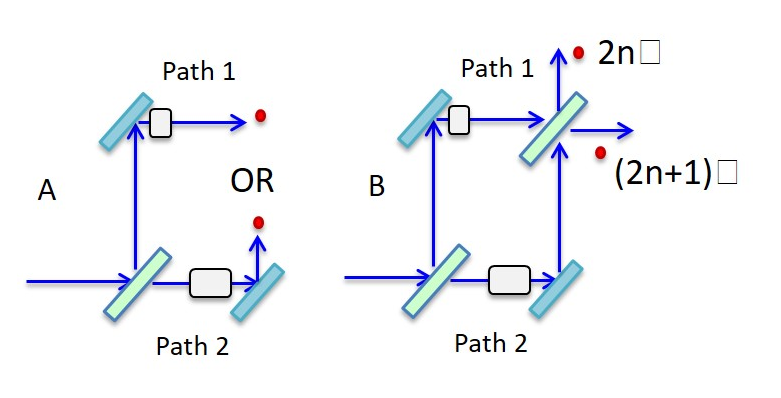
\includegraphics[scale=0.75]{src/images/chap27/1.eps}
\caption{FIG. 1: Proof against a matter-wave in real space: A) While the fact of detection as a particle is
unambiguous, any proposal of matter-wave in both paths, with each branch possesing the entire
mass, charge etc. violates all conservation laws. B) However, there is clear empirical evidence for
a physical entity, which is not a matter-wave, that is present in both paths in space, for every
particle. The evidence is in the fact that the observable state at the output port depends on what
physical element or interaction is present in both paths, for every single particle.}
\end{figure}


Having made the seemingly incredible assertion that there are no matter-waves in real
physical situations of quantum mechanics, one is obliged to give some empirical support to
the claim, apart from the demonstration in the derivation of the Schrödinger equation. This
is in fact easy. Consider the configuration of a Mach-Zehnder interferometer for atoms with
widely separated paths. The $\psi$-function of quantum mechanics gives the correct results for
all observable features, whether it is in the individual paths or in the interference zone, after
the beam-combiner. The $\psi$-function splits at the beam splitter, to be divided in the two
paths. But, what is clear is that the particle cannot be in both paths without violating
all fundamental conservation laws! Associated with each branch of the $\psi$-function, there is
the intrinsic properties of the particle in full (mass, electric charge, spin etc.), not divided
or smeared out. Therefore, a virtual copy in each branch would violate the conservation
laws, and a division of any sort would not be consistent with the general empirical results.
Therefore, it should be obvious that the $\psi$-function is not the matter wave, even in this
simple single particle situation. But, the $\psi$-function is all what is required to reproduce
all observable results. Hence, we can conclude that no matter-wave is involved in quantum
mechanics \cite{chap27-key2}. Instead, what is present as the $\psi$-function is an ensemble entity. Therefore,
we need to find a missing element; it is operative in each dynamical history, but it is not
the nonexistent matter-wave or the ensemble $\psi$-function!

In fact, the exact context in which the wave character is apparent in dynamics was
mentioned by Einstein, in his article `Physics and Reality' [3]: ``Experiments on interference
made with particle rays have given a brilliant proof that \textit{the wave character of phenomena of
motion} as assumed by the theory does, really, correspond to the facts." I have italicized the
crucial phrase; the wave character is not of the matter, but of the `phenomenon of motion'.

In the same article, Einstein stated another crucial insight about the $\psi$-function, which I
proved now from the analysis of the Schrödinger equation. Einstein wrote, “The $\psi$-function
does not in any way describe a condition which could be that of a single system; it relates
rather to many systems, to `an ensemble of systems' in the sense of statistical mechanics.
If, except for certain special cases, the $\psi$-function furnishes only statistical data concerning
measurable magnitudes, the reason lies not only in the fact that the operation of measuring
introduces unknown elements, which can be grasped only statistically, but also because of
the very fact that the $\psi$-function does not, in any sense, describe the condition of one single
system. The Schr\"{o}dinger equation determines the time variations which are experienced
by the ensemble of systems which may exist with or without external action on the single
system." It cannot be stated more transparently.

It is now clear why quantum mechanics has only statistical predictions; the simple reason
is that its fundamental equation is an equation for the evolution of the probability density.
But, we have not yet touched the cardinal feature of quantum mechanics, the phenomenon
of interference of dynamical possibilities. Why is the probability density structured with
interference? How can it happen without a `wave'? What is the reason for the intrinsic
irreducible uncertainty? We will discuss and answer these questions now.

\section{Then, What is the Equation of Dynamics?}%% 4

Having shown that the Schrödinger equation is not the dynamical equation, we have
the new task of finding the equation that governs the single particle dynamics. Of course
we know empirically that it cannot be very far from Newton's equation, which may also
be expressed in its Lagrangian form or the Hamiltonian form. Since, we found that the
hybrid character of the $\psi$-function involves the action, we now focus on its physical role
and proceed. Here, we need to go all the way back to W. R. Hamilton's insightful paper
in 1832 that introduced the principle of stationary action, generalizing from Fermat's least
action principle for optics \cite{chap27-key5}. In that paper, he developed a universal and ``general method
for expressing the paths of light, and of the planets". Hamilton also discussed the rationale
involved in the principle, through Huygens' theory of wave optics. In the subsequent papers
\cite{chap27-key6} that described the method for mechanics based on the `characteristic function', or the
action function $S(x, t)$, he wrote the general equation for dynamics as
\begin{equation*}
\frac{\partial S}{\partial t} = -H, \quad H = T + V  \tag{23}
\end{equation*}

The momentum is derived from the action as $\partial S/ \partial x = p$. The equation was called the
Hamiltonian equation by C. G. J. Jacobi, who developed it further mathematically \cite{chap27-key7}.
However, this equation does not explicitly acknowledge the original physical feature of action
that was the core reason for its property of being `stationary' or, extremal! The central
property that enables interference, which results in the dynamics along the path of stationary
action, is precisely \textit{the physical manifestation of action as a wave-like entity}. Otherwise, there
is no way the dynamical possibilities can cancel each other. The principle is operative because
the action is physically manifest in a wave property where the phase of the wave is the scaled
action. With this insight, the entire path is clear. As it stands, the Hamilton's equation
is not complete. Instead of an equation for the action, the correct and complete equation
that incorporates the Huygen's principle should have been for an oscillatory function of the
action. Hence, I complete Hamilton's action mechanics by modifying the equation to a new
universal form \cite{chap27-key2}
\begin{equation*}
\frac{\partial \zeta(S)}{\partial t} = - \frac{i}{\epsilon} H \zeta \tag{24}
\end{equation*}
where the function $\zeta(x, t) = \exp(iS(x, t)/\varepsilon)$. I call this function the `action-wave', since it
has a direct physical presence. This equation is the key step in the correct description of a
single particle, of a single dynamical history, in the reconstructed universal dynamics. The
parameter $\varepsilon$ is the fundamental scale of action that is to be determined empirically. This
equation contains Hamilton's equation $\partial S/\partial t = -H$.

The form of this single particle equation, without an ensemble `probability amplitude'
$A = + \sqrt{\rho}$ in it, shows why there was the prevalent confusion about the Schr\"{o}dinger equation
as a dynamical equation. The similarity is only partial though. This equation for the
time evolution of action does not involve the average over the ensemble. The Schr\"{o}dinger
equation is for the time evolution of a different entity, $\psi = \sqrt{\rho} \exp(iS/\varepsilon)$, represeting the
whole ensemble.
\begin{figure}[H]
\centering
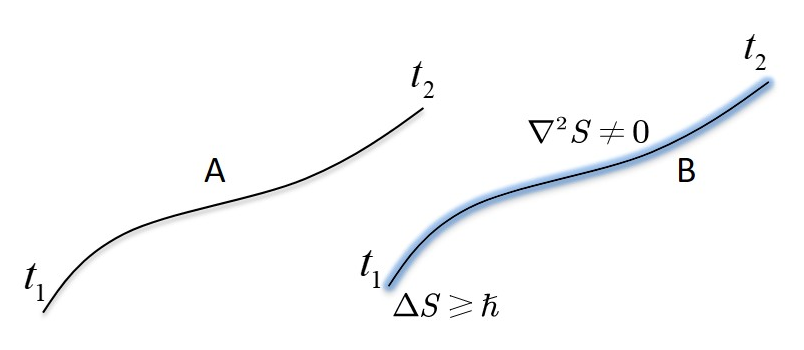
\includegraphics[scale=0.65]{src/images/chap27/2.eps}
\caption{FIG. 2: The difference between the path in the conventional Hamiltonian dynamics (A) and in
the new universal mechanics (B). In both schemes, the path has the stationary action $\delta S = 0$.
But factually, as indicated in the panel (B), the path has the intrinsic uncertainty $\Delta S \geq \hbar$ and a
nonzero concentration of action $\nabla^2 S$, which drives the diffusion (dephasing) of the action.}
\end{figure}

\textit{The first feature I note is that the action-wave is necessarily complex valued}. For, the relation between the first order time evolution and the Hamiltonian involves second order spatial
derivatives. Therefore, the dynamical equation cannot be built on a real periodic function
like cos($S/\varepsilon$) or on a real linear combination of sinusoidal functions; the action wave needs
both quadratures as a complex valued function, $cos(S/\varepsilon) + i \sin(S/\varepsilon)$. This is easily seen for
a constant potential, $H = V$. If $\zeta(S) \sim \cos (S/\varepsilon)$, then $\partial \zeta/\partial t \sim \sin (S/\varepsilon) \partial S/\partial t$, whereas
the right side is just $iV \cos (S/\varepsilon)$, which does not make sense. Therefore, the fundamental
equation for dynamics involves complex numbers because complex valued action waves are
the basis of dynamics at all scales. This feature is then \textit{inherited} by quantum mechanics.
The action-wave has unit amplitude, dictated by the dynamical equations $\partial S/\partial t = -H$ and
$\partial S/\partial x = p$.

We note the immediate main result that the new Hamiltonian action-wave equation
predicts intrinsic indeterminism in dynamics at all scales. The fact that the action is
involved in dynamics in the form $\exp(iS/\varepsilon)$ implies that the action is specified only up to
the scale $\varepsilon$. This does not mean that the action cannot be smaller than $\varepsilon$ or that it cannot be
arranged to be of a precise value in some dynamical arrangement. What I mean is that the
action $S$ is uncertain to $\varepsilon$ when no specific arrangement is made to define it precisely. This
will be explained quantitatively, with an example, later. Then, the equation itself contains
the stochastic element. With $H = (p^2 /2m) + V$, and $p = \partial S/\partial x$ we get,
\begin{align*}
i \varepsilon \frac{\partial \zeta (S)}{\partial t} & = \left(-\zeta \frac{\partial S}{\partial t} \right) = \left(-\frac{\varepsilon^2}{2m} \nabla^2 + V \right) \zeta = \zeta \left(\frac{p^2}{2m}  + V\right) - \zeta \frac{i\varepsilon}{2m} \nabla^2 S \tag{25}\\
\frac{\partial S}{\partial t} & = - H + \frac{i \varepsilon}{2m} \nabla^2 S\tag{26} 
\end{align*}

In addition to the familiar Hamiltonian mechanics in the first term, there is an additional
term proportional to $\varepsilon$ and to the \textit{concentration of the action in space}, $\nabla^2 S$. The equation
is the single particle, single dynamical history equation. Hence, this term points to the
variations in an ensemble of action-waves, for the dynamics of a single particle. \textit{When $\varepsilon$ is
tiny, this term is negligible. But it will become significant for microscopic dynamics}. To see
this clearly, consider the situation when $p \simeq 0$, and no potential. Then, we get
\begin{equation*}
\frac{\partial S}{\partial t} = \frac{i\varepsilon}{2m} \nabla^2 S \tag{27}
\end{equation*}

Though this resembles the diffusion equation, there is only one particle here and there is no
real diffusion possible. Also, the diffusing variable is not a density of particles here! What
is diffusing is the action itself. (Note that this is not the Schr\"{o}dinger equation, though it
resembles it. This is an equation for action when the Hamiltonian is zero). Now we see what
is the source of the small term diffusion-like time evolution of the probability amplitude,
$D \nabla^2 A$, with the imaginary diffusion constant $D = i \hbar /2m$. The dephasing of the action
waves in the equation 27 is the reason for that term.

The physical picture of new dynamics is then the following. The particle is indivisible,
and always localized. It has a dynamics determined by the action, with $\nabla S = p$, where
the action evolves according to the modified Hamilton's equation. The action is manifest in
dynamics as an entity with a periodicity defined by the scale $\hbar$. The action of the particle
(system) is defined with the intrinsic uncertainty of $\hbar$. The true and accurate statement of
the uncertainty principle, applicable to all scales of dynamics, is then $\Delta S  \geq \hbar$. The division
of $\Delta S$ into $\Delta p \Delta x$, $\Delta E \Delta t$ etc. are less precise statements of the fundamental uncertainty.
Since the action is the product of a dynamical quantity and the corresponding coordinate,
the division is justified, but it is not rigorous. The correct statement of the uncertainty
principle is just that the action is uncertain to $\hbar$ or larger.

The new equation of dynamics suggests that the wave in dynamics is then the wave
of action, represented by the function $\zeta (S) = \exp(iS/\varepsilon)$. Since we know from experiments
that there is some physical entity which encodes the physical characteristics of the particle
in the multiple paths (possibilities), it can only be the action wave. This is consistent will
all empirical facts and it has none of the vexing interpretational issues that people have
faced and are unable to deal with. Now let us see how every foundational physical issue of
quantum mechanics has dissolved away.

\section{Quantum Mechanics Without Collapse}%%% 5

The problem of the collapse of the $\psi$-function arose because the $\psi$-function was always
interpreted as representing a single dynamical history. Therefore, a state that is a superposition of two states like
\begin{equation*}
|\psi \rangle = a |S1 \rangle + b |S2 \rangle \tag{28}
\end{equation*}
was interpreted to become, or \textit{collapse to $|\psi' \rangle = |S1 \rangle$  or $|S2 \rangle$, in each realization of the
dynamics}. Then, the dynamics has to restart with a new $\psi$-function, causing discontinuity
in the Schr\"{o}dinger evolution. Also, when interpreted as a matter-wave, or anything related to a real presence in space, this reduction implies the instantaneous disappearance of such an entity from every other possibility, including different paths and locations in space. 
Therefore, the need for such collapse, in standard QM, is a severe unresolved problem.

However, I have shown now that the $\psi$-function pertains to the ensemble. Then, it is
clear that there is no `superposition' of the \textit{states of the particle}, nor is any reduction of
the function during each observation; a probability density of the ensemble does not change
during each realization of its possible stochastic results! The superposition is only for the
action waves, and not for the physical state of the particle. This single physical feature
of the new mechanics is the only central fact to be understood for the solution of any
foundational issue. The particle is either in the state $|S1 \rangle$ or in the state $|S2\rangle$, and never
in a superposition, in each dynamical history, and that is what we observe. I reiterate that
a superposition of particle (matter) states blatantly violates all conservation laws, because
a general superposition would then include formally (mathematically) the situation of the
particle being in two spatially separated paths. The particle is already in the path where
it is observed, with an uncertainty of its action amounting to $\hbar$, and only that much. The
detection of the particle interrupts only the action wave in that particular path. It does not
cause any change in the propagation of the action waves in any other possibility. Since the
action waves carry only action, and no energy or momentum, none of the physical quantities
needs the reassigning, as it is necessary in standard quantum mechanics with the device of
the `collapse of the wavefunction'. We have solved the core difficulty of standard quantum
mechanics and have removed its fundamental arbitrariness and discontinuity. Now we need
to verify that the core property of interference happens because of the overlap of the action
waves in the two paths. This is the step that was missing from Einstein's advocacy of the
interpretation of the $\psi$-function as pertaining to the ensemble.

The coefficients in the $\psi$-function are $a = + \sqrt{\rho_1}$ and $b = + \sqrt{\rho_2}$ (the sign from any phase
belongs to the action waves and not to the real amplitudes, which are ensemble quantities).
Here the (discrete) probabilities $\rho_1$ and $\rho_2$ that determine the division of the particles in the
two possibilities depend on the experimental configuration, like the width of the slits etc.
The same configuration determines the division of the action as well, into $ae^{iS/\hbar}$ and $be^{iS/\hbar}$.
After the dynamical evolution, the action waves combine as
\begin{equation*}
\zeta(S) = ae^{iS(a)/\hbar} + be^{iS (b)/\hbar} \tag{29}
\end{equation*}

The intensity is
\begin{align*}
\zeta (S) \zeta (S)^{\ast} & = a^2 + b^2 + abe^{-iS (a) /\hbar + iS (b)/\hbar} + abe^{+ S (a)/\hbar - iS (b)/\hbar}  \\
& = a^2 + b^2 + ab \left[e^{\frac{i}{\hbar} (S(b) - S(a))} + e^{\frac{i}{\hbar}(S(b) - S (a))} \right] \tag{30}\\
& = \rho_1 + \rho_2 + 2 \sqrt{\rho_1 \rho_2} \cos  (S (b) / \hbar - S (a) / \hbar) \tag{31}
\end{align*}

We see that the particle ensemble density follows the intensity of the action waves $|\zeta(S)|^2$,
and the entire probability from 0 to 1 is mapped to the tiny scale of action $\hbar$. In these physical
situations, the action is typically of the form $S = \int p_i dx^i$, where $p_i$ is a dynamical variable
like the energy, momentum or spin, and $dx^i$ is the corresponding (conjugate) coordinate.

I have solved explicitly what Feynman stated as the ``only mystery" of QM; the observation of
 particles is as a single whole, localized, and yet the interference phenomena happen
by the accumulation of the single quantum histories that depends on all the dynamic possibilities available to every particle, taken one by one.


\section{Quantum Mechanics Without the Measurement Problem}%% VI

The solution of the problem of collapse solves also the most discussed `quantum measurement problem' \cite{chap27-key8} as well, because that physical problem in QM concerns the collapse of the joint $\psi$-function of a particle and another physical system, called the `apparatus', which is
formally identical to the $\psi$-function of a `two-particle' system. The solution is very easy to
state: in each instance of observation, the particle is exactly in one of the possible physical
states. The apparatus observes the factual state, after the interaction with the particle,
with the possible uncertainty in the action $\Delta S \approx \hbar$. If $|s_a  \rangle$, $|s_b\rangle$, $|s_c\rangle...$ are the possible
states and $|A_a \rangle$, $|A_b \rangle$, $|A_c \rangle ...$ the corresponding apparatus states, each observation results in
only one correlated state, $|s_i \rangle ~|A_i \rangle$, because the particle is factually in just one of the states.
Different realizations happen $|s_a \rangle ~ |A_a  \rangle$, $|s_b  \rangle | A_b \rangle$ etc., with probability $p_a = a^2$, $p_b = b^2 ...$ etc.
Obviously, the ensemble probability density function ($\psi$-function) is
\begin{equation*}
|\Psi \rangle = a | s_a \rangle | A_a \rangle + b |s_b \rangle | A_c \rangle \ldots + n | s_n \rangle | A_n \rangle \tag{32}
\end{equation*}

Being an ensemble entity, this does not collapse when any particular observation is realized.

Though \textit{the quantum measurement problem is completely solved}, as I just showed, we are
yet to show the correct treatment of the interference phenomena in the two-particle state,
which holds the additional puzzle on `nonlocality', because the two systems (the two particles
or the particle and the apparatus) can be spatially separated, at two different locations, after
an interaction. The hard open problem of spatial nonlocality is in fact the most discussed
foundational issue, ever since the publication of the Einstein-Podolsky-Rosen (EPR) paper
\cite{chap27-key9}. We take up the quantum interference phenomena of two-particle states in QM next.

\section{The Two-Particle Correlation}%% 7

It is very instructive to consider the $\psi$-function of two particles. The realization that the
$\psi$-function of QM pertains to the ensemble, and not to a single dynamical history of two
particles, drastically changes our understanding of the entangled state in QM. An example
is convenient. The spin-singlet state is
\begin{equation*}
|S\rangle = \frac{1}{\sqrt{2}} (|u \rangle_1 | d \rangle_2 - | d \rangle_1 |u\rangle_2) \tag{33}
\end{equation*}

As we just discussed, this ensemble description corresponds to two classes of joint states
happening randomly, with equal probability, $|u \rangle_1 |d \rangle_2$ and $|d \rangle_1 |u \rangle_2$. These are the factual
states, and exactly one of them represents each occurrence of a dynamical history. As far
as the particle states are concerned, there is no superposition. In fact, that is why there
is no quantum measurement problem. However, the action waves corresponding to the two
distinct joint states can of course superpose and interfere, resepecting strictly locally. An
action wave at one location cannot interfere with an action wave at another location. Hence,
strict locality is obeyed by the action waves as well as the particles. Do I get the two-particle
correlation correctly?
\begin{figure}[H]
\centering
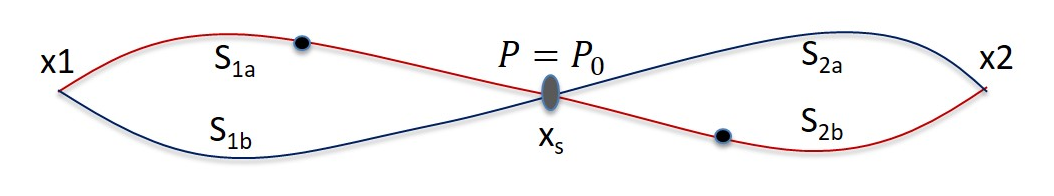
\includegraphics[scale=0.55]{src/images/chap27/3.eps}
\caption{FIG. 3: Two-particle correlation from the strictly local interference of the correlated action waves at
locations $x1$ and $x2$. The source obeys a dynamical constraint, represented by $P = P_0$ here, which
reflects in the action $S_{1a}, ~S_{2b}$ etc. The particle dynamics is definite and completely separable in
each pairwise event. The property of entanglement is an apparition created due to misinterpreting
the ensemble entity $\psi$ as a representation of single quantum history.}
\end{figure}

I am aware how unbelievable it would be to most if the two-particle correlations emerged
correctly from strictly local interference phenomena in mechanics. This is because there is a
prevalent belief that quantum correlations emerge from a nonlocal influence passing between
the particles, even though there is not even an iota of empirical evidence in support of this
belief. The reason for this unfounded belief is explained in a later section, for completeness.
The explicit derivation now will anyway prove that such a belief is misplaced. Presently, I
derive the two-particle correlation from the local interference of the action waves, respecting
strict Einstein locality. For clarity, I consider the case of two physical possibilities $a$ and $b$
for each particle, which could be two spin projections or two paths in an interferometer etc.
(figure 3).

For a general two-particle state, each dynamical history is characterized by the action waves
\begin{align*}
\zeta_{1a} & = e^{iS_{1a}/\hbar}, \quad \zeta_{1b}  = e^{iS_{1b}/\hbar} \tag{34}\\
\zeta_{2a} & = e^{iS_{2a} /\hbar}, \quad \zeta_{2b} = e^{iS_{2b}/\hbar} \tag{35}
\end{align*}

However, if a dynamical resource $p$, like the energy, momentum, spin etc., of the two particles
together is fixed, say as $p = 0$, to be shared between the two particles, then $p_1 = - p_2$ (the
action is $S = \int pdx$). The action waves interfere at the location of the observations on the
first particle as
\begin{equation*}
\zeta_1 = \frac{1}{\sqrt{2}} e^{iS_{1a}/ \hbar}  + \frac{1}{\sqrt{2}} e^{iS_{1b} /\hbar} \tag{36}
\end{equation*}
with intensity, $\zeta_1 \zeta_1^{\ast}$,
\begin{align*}
\zeta_1 \zeta^{\ast}_1 & = \frac{1}{2} \left(1+1+e^{-iS_{1a}/ \hbar} e^{iS_{1b} / \hbar} + e^{iS_{1a} / \hbar} e^{-iS_{1a}/\hbar} \right)\\
& = \frac{1}{2} \left( 1+1+e^{i(S_{1b} - S_{1a})/\hbar} + e^{-i(S_{1b} - S_{1a}/\hbar)} \right) = 1 + \cos (S_{1b} - S_{1a})/\hbar \tag{37}\\
& = 1 + \cos (p_{1b} (x-x_s) - p_{1a} (x-x_s)) / \hbar = 1 + \cos \Delta p (x-x_s) /\hbar \tag{38}
\end{align*}

Though this expression resembles the familiar interference formula, there is no stable interference because of the presence of the source coordinate $x_s$, with an uncertainty $\hbar/ \Delta p$ corresponding to the uncertainty $\hbar$ in the action of the individual particle. Therefore, I can
now predict that \textit{the maximally correlated state does not show any single particle interference}. This is why the measurements at each location gives random results for any fixed setting `$x$' of the apparatus.

What is the result for the correlated observation on both the particles? This is the
central problem of `quantum correlations'. The crucial physical point in the joint measurements is the correlated nature of the action waves corresponding to the two particles, with a constraint on the total quantity of a dynamical variable. While there are four joint possibilities for the physical processes (two each for each particle), only two can manifest in the correlation-constrained case, with $p_1 = -p_2$. Then the only two action wave combinations
are $e^{iS_{1a} /\hbar}  e^{iS_{2b} /\hbar}$ and $e^{iS_{1b}/ \hbar} ~e^{iS_{2a}/\hbar}$. The other two possibilities cannot occur due to the
constraint (conservation laws). The joint presence of these action waves then interfere, but strictly locally, at location 1 and 2 separately.
\begin{align*}
\zeta_1 \zeta_2 & = \frac{1}{\sqrt{2}} e^{ip_{1a} (x_1- x_s) /\hbar} e^{ip_{2b} (x_2 -x_s) /\hbar} + \frac{1}{\sqrt{2}} e^{ip_{1b} (x_1 - x_s) /\hbar} e^{ip_{2a} (x_2 - x_s) /\hbar}  \tag{39} \\
& = \frac{1}{\sqrt{2}}  \left(e^{ip_{1a} (x_1- x_s) /\hbar} e^{-ip_{1a} (x_2 -x_s) /\hbar} + e^{ip_{1b} (x_1 - x_s) /\hbar} e^{-ip_{1b} (x_2 - x_s) /\hbar} \right) \tag{40}\\
& = \frac{1}{\sqrt{2}} \left[ e^{ip_{1a} (x_1- x_2) / \hbar} e^{ip_{1b} (x_1 -x_2) /\hbar}  \right]
 \tag{41}\\
\end{align*}

\textit{The correlation in the action waves from the common source eliminates any dependence on
the source coordinate}, and thereby the initial uncertainty and randomness of the action! The
distribution of the results of joint measurements are then given by the quantity
\begin{align*}
|\zeta_1 \zeta_2|^2 & = \frac{1}{2} \left[e^{-ip_{1a} (x_1 -x_2)/\hbar} + e^{-ip_{1b} (x_1-x_2)/\hbar} \right] \left[e^{ip_{1a} (x_1 -x_2) /\hbar} + e^{ip_{1b} (x_1 - x_2)/\hbar} \right] \\
& = \frac{1}{2} \left[1+1+e^{-i(p_{1a} - p_{1b}) (x_1-x_2)/\hbar } + e^{i(p_{1a} -p_{1b}) (x_1-x_2)/\hbar} \right]\\
& = 1 + \cos (p_{1a} - p_{1b}) (x_1 -x_2) / \hbar = 1 + \cos \Delta p (x_1-x_2) / \hbar
\end{align*}


I have derived the two-particle quantum correlations assuming strict locality! The same
derivation, when the dynamical variable is the spin, reproduces the correct spin correlation
$C(\theta) - \cos \theta$ \cite{chap27-key2}. This is a remarkable general result for several reasons. It shows that
the physical state of each particle is definitely one of the two possibilities, correlated with
a definite state of the other, in each instance, with absolutely no inseparability, entanglement, or nonlocal feature. The property of entanglement is an apparition created due to misinterpreting the ensemble entity, the $\psi$-function, as a representation of the single quantum history. The correct two-particle correlation is the result of the local interference of the correlated action waves. The derivation shows transparently that the correlation follows causally from the conservation constraint on the common source of two particles, with no element of unphysical nonlocality. This single result restores causality and locality in
physics.

The derivation of the two-particle correlation respecting strict locality clarifies also that
my discussion of the Schrödinger equation and the action wave have no relation whatsoever
with a well-known attempt by D. Bohm to construct a deterministic quantum theory, with
the Schrödinger equation and its wavefunction as its basis for the description of a single
dynamical history \cite{chap27-key10}. It had its roots in an earlier theory by de Broglie, in which the
‘wave' was considered to `pilot' the particle; thus the wave and particle were separated to
some extent, but the physical nature of the wave could not be clarified. Also, Bohmian
mechanics is very nonlocal in nature. The theory splits the Schr\"{o}dinger equation into two
parts: one is the `classical' Hamilton-Jacobi equation for the evolution of action, now with
a quantum potential, and the other is the continuity equation for the real square root of
the probability density. Then, the gradient of the action $\nabla S(x, t) = p$ is interpreted as the
guiding equation for the particle, with the position variable as a real but hidden parameter.
Then, each trajectory is known, given the initial position and the action function, as in the
usual Newtonian dynamics. However, the theory has the nonlocal quantum potential that
depends on the position of all particles in a multi-particle situation. The theory inherits its
unphysical features from treating the Schr\"{o}dinger equation as the equation of dynamics for
the single quantum history, which is what is shown to be incorrect in this paper. Einstein
himself had showed a gross unphysical feature of Bohm's theory, even for a single particle
situation of a macroscopic particle in a box \cite{chap27-key11}.

\section{Summary of the main Results}%% 8


I have completed the presentation of the main results of the new universal mechanics,
applicable to all scales, without any distinction of microscopic and macroscopic, or relativistic and nonrelativistic dynamics. The classical-quantum division was entirely artificial, as hoped by many, but never demonstrated earlier. With the completion of the Hamilton's action mechanics, with the equation of dynamics written for a wave function of action rather than for the action, the inconsistent proposal of the matter-wave is eliminated from mechanics. Both causality and locality are restored in microscopic dynamics, and the tiny intrinsic indeterminism is traced to the scale of the action wave. A summary of the main results is in order.

I started with a review of how the Schr\"{o}dinger equation came about, and became the
working equation of quantum mechanics. Then I argued that the equation could not be
interpreted as the equation for dynamics, because the $\psi$-function could not be related to
any dynamical variable or to any entity associated with de Broglie's matter-wave in space.
Then I showed in detail that the Schr\"{o}dinger equation is in fact the (continuity) equation
for the time evolution of the complex square root of the ensemble probability density of a
dynamical system, and the $\psi$-function is just this ensemble entity. Thus the equation does
not pertain to the dynamics of the single particle or a single dynamical history. The equation
of dynamics only serves as the constraint to define that the probability density pertains to
a dynamical system. This analysis also proved that the Born's rule is an exact requirement,
by the definition of the $\psi$-function, and not an additional rule.

As the next step, I showed empirical evidence that de Broglie speculated matter waves
cannot be any part of the theory of quantum mechanics because matter in superposition
violates all conservation laws. Then I argued, again from experimental situations, that there
is a definite physical entity, which is not the matter wave, that is present in the multiple
possibilities of quantum dynamics, with the dynamical evolution of the localized particle. This has the periodicity properties of a wave.

The demonstration that the Schrödinger equation is not the equation of dynamics implied
the existence of a new universal equation for single dynamical histories. This was derived
next, as a modified Hamilton's equation, for a periodic function of the action. This was
logically necessary since the only physical reason why the principle of stationary action
is operative in all dynamics, is the wave property associated with the action. Hence, the
original Hamilton's equation that did not incorporate this explicitly was incomplete. Then
the structure of the new equation immediately resulted in two fundamental results; 1) there
is an intrinsic irreducible indeterminism for all scales of dynamics with a comprehensive
uncertainty principle, $\Delta S \geq  \hbar$, 2) the action wave (function) is necessarily complex valued,
because the Hamilton's equation relates a first order differential evolution in time, of the
action wave, to its spatial derivative of second order, and also constant multipliers. The
new equation contained the standard Hamilton's equation along with the new term that
governed the intrinsic stochastic element in dynamics, containing the constant $\hbar$.

Then I showed that the vexing problem of the collapse of the quantum state and the
wavefunction was absent in the new mechanics! The dynamics of the particle is definite, in
just one of the possible states, and the physical state of the particle is never in any superposition of states. Particle states do not superpose; only action waves can superpose. But, they do not have the problem of collapse during quantum measurements. Then an explicit
calculation showed that the central phenomenon of interference is reproduced correctly by
the action waves, without any need for matter waves and superposition of particle states.
Extending the notion and the calculation to two systems, either of two particles or a particle and a measuring apparatus, I showed that the important open problem of quantum
measurement is entirely solved. Next, I showed that the $\psi$-function of a two-particle system, being the representation of the probability density associated with the ensemble and not individual pairs, has none of the bizarre properties attributed to the entanglement of
particle states. The pair of particles is in definite correlated states in each event, and only
the action waves corresponding to the multiple possibilities are in correlated superpositions.

Finally, I took up the hard problem of two-particle interference and correlations. A simple
calculation then demonstrated that the two-particle correlations are correctly reproduced by
the strictly local interference of the action waves. Thus, there is no alleged nonlocality in
the correlations of the `entangled' states.

This last result goes counter to the widely held conviction that telepathic nonlocal influences are a fact of the quantum world. Therefore, it remains to show that this is a wrongly held belief about the two-particle correlations in the conventionally entangled states. Since I have already provided explicit and transparent proofs that Einstein locality is strictly respected by the two-particle correlation, there is the urgent duty to show clearly the exact reasons for the unfounded beliefs. I aim complete clarity and no room for ambiguity in this task, which I will now take up, in a brief discussion.

\section{Some Comments on Nonlocality and Bell's Hidden Variables}%%9

Many people think, and express their conviction, that the correlation of spin projections
seen in the case of certain two-particle states, like the spin-singlet, is nonlocal, in the sense
that the result of the observation at location A acts as the physical cause of the result at
another location B, instantaneously propagating from A to B. Thus, they assert that any
theory that correctly reproduces the result is also nonlocal, allowing such influences in the
structure of the theory. The reason given by the people who believe in this is the Bell's
theorem and the Bell's inequality. If the reader is a believer, then a very careful and calm
reading is prescribed, after which the belief will not stay.


Bell's inequality \cite{chap27-key12} was derived in the context of the local hidden variable theories
(LHVT), which have nothing to do with quantum mechanics. They are a class of `classical'
statistical theories in which all observables are factually present with definite values for a
physical system, but the measurement shows the quantized and stochastic result, consistent
with the quantum state, due to the unknown stochastic values taken by a set of hidden variables (which are not identified, physically). These theories assume locality. Bell's inequality deals with the correlation between the quantized observables $A_i = \pm 1$ and $B_i = \pm 1$ on two
entangled particles, measured at locations A and B. The inequality (or the theorem) is the
statement that a certain combination of the two-particle correlation $C (\theta)$ is bounded by a
strict upper limit (the parameter $\theta$ is the relative setting of the relevant parameters in the
measurement, like an angle for the spin direction). It can also be stated as the specific linear
form of the correlation function in the LHVT. This upper limit is violated by the results
obtained in actual experiments, by a large margin. Therefore, the (only) natural logical
conclusion is that the LHVT are not tenable as physical theories. Nobody who practises
logic as usually used in science would conclude that a natural phenomenon is nonlocal, from
the experimental result that the two-particle correlation is larger than the upper limit set
by an arbitrary fringe theory, in which the assumption of locality was used! However, unbelievably, that is exactly what happened. After the demonstrated failure of the LHVT,
people concluded that the assumption used in an alternate theory is violated in nature. In
other words, it was implied that the LHVT would be the correct kind of theory, if only its
assumption of locality is removed. That is entangled logic indeed.
\begin{figure}[H]
\centering
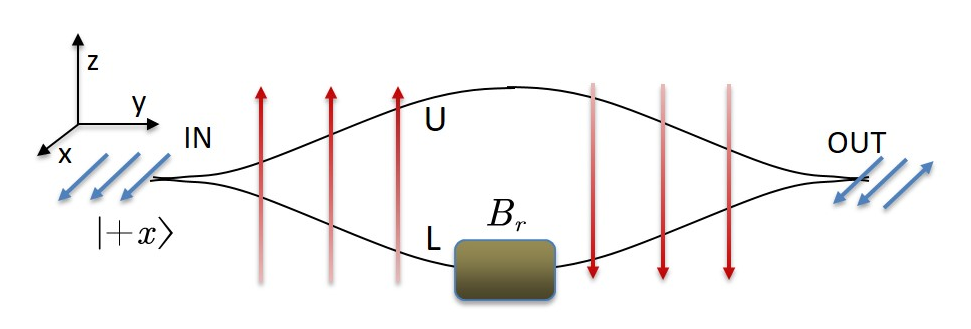
\includegraphics[scale=0.55]{src/images/chap27/4.eps}
\caption{FIG. 4: The measurement of a spin component after a Stern-Gerlach interferometer. The input spin
is polarized along $+x$. In the hidden variable scheme, each particle, with all its spin components,
is either in the upper path or in the lower path, with equal probability. Therefore, the spin rotator
$B_r$ affects only half the particles. In contrast, the phase factor in the lower path affects all the
particles according to QM. Bell's hidden variable scheme fails here.}
\end{figure}

If there is any lingering doubt, let me establish two facts that are devastating for what
has been done in the context of the LHVT, both in the theory and experimental tests: a)
Bell's well known demonstration \cite{chap27-key12}, \cite{chap27-key13} of a `successful' hidden variable scheme for the
measurements of a single quantum spin is faulty and fails miserably, discrediting the entire
LHVT enterprise. b) the LHVT considered by Bell and tested as a viable theory by many
are in fact unphysical theories because they grossly violate fundamental conservation laws
\cite{chap27-key14}, \cite{chap27-key15}!

In an argument countering J. von Neumann's proof that the hidden variable theories can-
not mimic quantum mechanics, Bell showed that the measurement of a spin-1/2 projection
along any direction $\vec{a}$ for the state polarized along $\vec{n}$ can be reproduced correctly in a simple
hidden variable scheme. Then, one reproduces the eigen-results of only $+1$ and $-1$, irrespec
tive of the direction $\vec{n}$, with the correct average $\vec{n} \cdot \vec{a}$.
 The hidden variable in this case was another vector that took all directions about the vector $\vec{n}$ randomly, which is averaged to
get the expectation values. Let us quickly see the fundamental fault with any such scheme.
If the direction of measurement coincides with the polarization direction, then all the results
would of course be $+1$. Let $\vec{n} = + \hat{x}$. We have set $\vec{a} = + \hat{x}$. All the particles in the state
$|+x \rangle $ have their spin value along $+ \hat{x}$ as $+1$. In the LHVT, the other two components along
$\hat{y}$ and $\hat{z}$ directions take one of the values $+1$ and $-1$, randomly for each particle, whereas in
QM, these values cannot be specified (indeterminate). So far, Bell's LHVT gives the same
results as QM. Now, I introduce a symmetric Stern-Gerlach splitter and combiner, aligned
for the $+z$-direction, in between the source of the particles and the measurement apparatus
(figure 4). This does not change anything in the measurement results. However, now the
LHVT has no choice but to admit that half the particles take the upper path in the SG
section and the other half, the lower path. No spin component is altered by the scheme as
long as the `spin-rotator' $B_r$, with the localized magnetic field in the lower path of the SG
section. is not operated. This device rotates the spin by a full $2\pi$ angle, back to the initial
direction. The spin components in the upper SG path are not affected.

What is the prediction for the values for the spin components in Bell's hidden variable
scheme? Without going into any details, we see that certainly nothing changes for half the
particles; they will be measured as $+1$ in the $+ \hat{x}$ direction. However, the QM prediction is
very different! The $|+x \rangle$ state is the superposition,
\begin{equation*}
| + x \rangle = \frac{1}{\sqrt{2}} | + z\rangle + | - z \rangle \tag{42}
\end{equation*}

The spin rotator changes the phase of the $|-z \rangle$ state by $\exp(i \pi) = -1$. Then QM state after 
the SG section is
\begin{equation*}
|s \rangle = \frac{1}{\sqrt{2}} (|+z) + \exp (i \pi) | - z \rangle = | - x \rangle \tag{43}
\end{equation*}
\textit{for every particle. Therefore, the spin value of all the particles will be measured as $-1$, along
the $+ \hat{x}$ direction}. So, Bell's scheme fails, contrary to the general impression. The quantized
spin component is only one of the feature of a `state' in quantum mechanics; the phase of
the state determines the distribution particles. From the discussion earlier, we know that
this phase is that of the action waves.

Further, I will now show that the Bell's inequality itself is derived for a physically inad equate theory, which should not have been take seriously in the first place. Surely, people who spent enormous efforts in testing them would not have realized that the LHVT for the
spin-singlet violates the conservation of angular momentum!

The spin correlation concerns the measurements on two particles and the possible results
at locations A and B are $A_i = \pm 1$ and $B_i = \pm 1$. When both the measurements are in the
same direction, the angle between the apparatus directions, $\theta = 0$. Then, if $A_i = +1$, then
$B_i = -1$ and vice versa; only then the total spin is zero, as demanded by the conservation
of the angular momentum. To see what \textit{the empirical correlation is for a general angle,
dictated by just the conservation of the angular momentum}, consider the measurements at
A and B with the difference $\theta \neq 0$ in the angular settings. The correlation is the average of
a large number of products $A_i B_i$.

Since the average of a sum of quantities is the same as the sum of the averages of two
subsets that are half the size, we can make the subsets $A_i (+1)B_i$ and $A_i (-1)B_i$, where the
first set has all $A_i = +1$ and the second has all $A_i = -1$. Then the correlation function
determined by just the conservation laws, independent of any theory, is
$$
C_e (\theta) = \frac{1}{N} \sum A_i B_i = \frac{1}{N/2} \sum A_i (+1) B_i + \frac{1}{N/2} \sum A_i (-1) B_i
$$

This involves only a simple reordering of the pairs of data, keeping the pairwise data intact, which does not affect any average (we can do the same exercise with the B values as the anchor - the situation is symmetric). Now note that the first set has the average angular
momentum at A as $+1$ and the second set as $-1$ (in units of $\hbar/2$). Then, the conservation
of the angular momentum on the average dictates that the corresponding average value at
B, at a relative angle $\theta$, should be the projection of the opposite angular momentum along
the direction of B; in the first set it should be $- \cos \theta$ and in the second, $+ \cos \theta$. Then the
average for the whole set is just
\begin{equation*}
C_e  (\theta) = (+1 \times -\cos \theta) + (-1 \times + \cos \theta )  = - \cos \theta \tag{44}
\end{equation*}

This is predicted to be the experimentally observed singlet correlation, purely from the
conservation of the angular momentum, independent of any theory. A theory that has a
different prediction is then definitely not compatible with the conservation of the average
angular momentum. Obviously, such theories are unphysical. Since the LHVT predict a
very different correlation function that has a linear dependence on $\theta$ for small angles, the
LHVT are in that unphysical class. Will anyone wants to test them, or even discuss them,
once this result is known?!

One would have noticed that we did not even mention the EPR result about quantum
mechanics while discussing the severe problems with Bell's results. That is because Bell's
results are entirely in the realm of a class of classical statistical theories that have no relation
to quantum mechanics or to the EPR result. Usual discussions mix up issues and theories,
without an adequate logical and empirical judgement. Our discussion laid out the premises
and results with absolute clarity, and then showed how irrelevant the failure of the physically
faulty LHVT is for any discussion on the problems and peculiarities of quantum mechanics.


\section{Concluding Remarks}%%%10

This article was written for my own intellectual benefit. However, writing this required
the considerate invitation and the generous leeway of topic and time offered by the ``GR-
team", some members of which are my friends. My limited interactions with Prof. G.
Ramachandran were while he was an emeritus professor at the Indian Institute of Astrophysics, Bengaluru, where I was a frequent visitor. I discussed some aspects related to the
foundational issues, but his interest was mostly in applying the quantum formalism to physical problems, perhaps because he considered the theory as complete, and certainly adequate. I would have enthusiastically reported to him the conclusion that I now see, of the reasoned
`hunch' on quantum correlations and Einstein locality that I discussed then. Now, I have
the complete proof and derivations that establish the absence of nonlocality in quantum
correlations, along with a full understanding of how and why one strayed into an irrational
path. This is then that report, with the kind of logical integrity and the quantitative and
calculational details that he would have appreciated, I believe.

\begin{thebibliography}{99}
\bibitem{chap27-key1} E. Schr\"{o}dinger, An undulatory theory of the mechanics of atoms and molecules, Phys. Rev. 28, 1049-1070 (1926).

\bibitem{chap27-key2} C. S. Unnikrishnan, Reconstructing quantum mechanics without foundational problems, ArXiv:1812.06088.

\bibitem{chap27-key3} A. Einstein, Physics and reality, Journal of the Franklin Institute 221, 349-382 (1936); Quantum mechanics and reality (in German), Dialectica 2, 320-324 (1948).

\bibitem{chap27-key4} A. Einstein, Remarks to the essays appearing in this collective volume, in Albert Einstein: Philosopher-Scientist, A. Schilpp (Ed.) (MJF Books, NY, 1949).

\bibitem{chap27-key5} W. R. Hamilton, On a general method of expressing the path of light, and of the planets, by the coefficients of a characteristic function, Dublin University Review and Quarterly Magazine 1, 795-826 (1833).

\bibitem{chap27-key6} W. R. Hamilton, Second essay on a general method in dynamics, Philosophical Transactions of the Royal Society, part I, 95-144 (1835).

\bibitem{chap27-key7} M. Nakane and C. G. Fraser, The early history of Hamilton-Jacobi dynamics 1834-1837, Centaurus 44, 161-227 (2002).

\bibitem{chap27-key8} A. J. Leggett, The quantum measurement problem, Science 307, 871-872 (2005).

\bibitem{chap27-key9} A. Einstein, B. Podolsky, and N. Rosen, Can quantum mechanical description of physical reality be considered complete?, Phys. Rev. 47, 777-780 (1935).

\bibitem{chap27-key10} D. Bohm, B. J. Hiley, and P. N. Kaloyerou, An ontological basis for the quantum theory, Physics Reports 144, 321-375 (1987).

\bibitem{chap27-key11} A. Einstein, Elementary considerations on the interpretation of the foundations of quantum mechanics (a translation by D. Karanth, of Einstein's paper from `Scientific Paper Presented to Max Born on his retirement from the Tait Chair of Natural Philosophy in the University of Edinburgh', 1953), arXiv:1107.3701.

\bibitem{chap27-key12} J. S. Bell, On the Einstein-Podolsky-Rosen paradox, Physics 1, 194-200 (1964).

\bibitem{chap27-key13} J. S. Bell, Speakable and Unspeakable in Quantum Mechanics (Cambridge University Press, 1987).

\bibitem{chap27-key14} C. S. Unnikrishnan, Correlation functions, Bell's inequalities and the fundamental conservation laws, Europhys. Lett. 69, 489-495 (2005); arXiv:quant-ph/0407041

\bibitem{chap27-key15} C. S. Unnikrishnan, The incompatibility between local hidden variable theories and the fundamental conservation laws, Pramana-Jl. Phys. 65, 359-379 (2005).

\end{thebibliography}

